\section{Czy opłaca się powtarzać uruchamianie algorytmów LS?}
\begin{figure}[!h]
\centering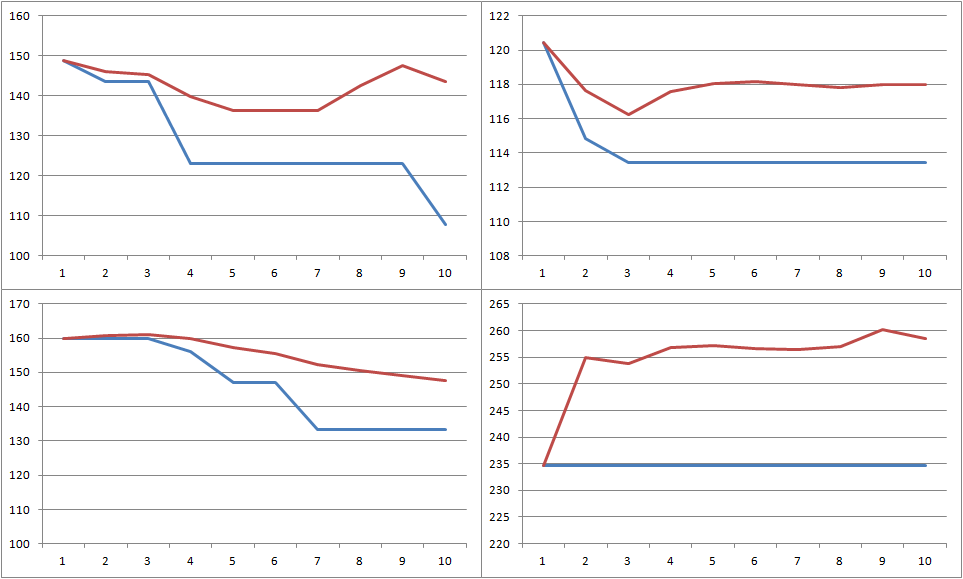
\includegraphics[width=12cm]{img/min_vs_avg_g.png}
\caption{Wykresy przedstawiające porównanie odnalezionej wartości minimum (kolor niebieski) względem wartości średniej (kolor czerwony) rozwiązania dla kolejnych odpaleń algorytmu Greedy dla instancji (w kolejności od góry do dołu, od lewej do prawej): br17, ft53, ft70, ftv170}\label{rys:mvsag}
\end{figure}
\begin{figure}[!h]
\centering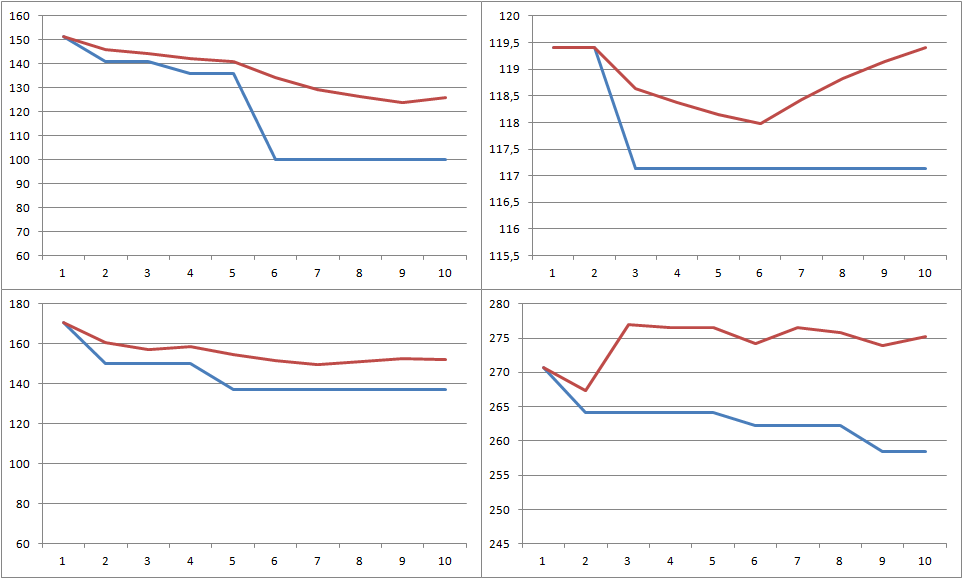
\includegraphics[width=12cm]{img/min_vs_avg_s.png}
\caption{Wykresy przedstawiające porównanie odnalezionej wartości minimum (kolor niebieski) względem wartości średniej (kolor czerwony) rozwiązania dla kolejnych odpaleń algorytmu Steepest dla instancji (w kolejności od góry do dołu, od lewej do prawej): br17, ft53, ft70, ftv170}\label{rys:mvsas}
\end{figure}

Na rysunku \ref{rys:mvsag} oraz \ref{rys:mvsas} przedstawiono porównanie dotychczas odnalezionej wartości minimalnej wzgledem średniej wartości odnalezionych rozwiązań w ramach kolejnyc odpaleń odpowiednio algorytmu Greedy oraz Steepest. Oczywiście wraz z kolejnymi odpaleniami wartość średnia jest zdecydowanie gorsza niż odnalezione minimum, co było spodziewanym efektem. Zauważyć można, że jeśli w danej iteracji poprawiono minimum to wartość średnia również staje się mniejsza, co jest naturalne.

Przedstawione wykresy wskazują jednak nieco inną ciekawą właściwość, która dotyczy tak naprawdę liczby miast do odwiedzenia. Przy małej liczbie miast (do ok. 60) obydwa algorytmu co kilka iteracji są w stanie poprawić minimum co jest pożądane. Jednak przy większej ich liczbie algorytm Greedy skacze już zbyt chaotycznie, żeby uzyskiwać coraz to lepsze rezultaty. Natomiast Steepest w tym czasie dla instancji 170 miast był w stanie poprawić uzyskany wynik podobnie jak miało to miejsce dla mniejszej liczby miast.

Powyższe spostrzeżenie wynika z dwóch faktów. Po pierwsze liczba miast w problemie ma istotny wpływ na krajobraz rozwiązań i powoduje, że może istnieć więcej minimów lokalnych, w które trafia Greedy bardzo szybko. Z kolei drugi fakt to natura Steepest'a, który zawsze schodzi wybraną przez siebie najlepszą ścieżką od danego rozwiązania, dzięki czemu istnieje szansa, że szybciej trafi do tych bardziej korzystnych rozwiązań. Oczywiście to wszystko przy założeniu, że ten krajobraz jest faktycznie na tyle skomplikowany i poszatkowany, że tych wartości minimów lokalnych jest naprawdę sporo.

Niestety wydaje się, że mimo wszystko przez losowość punktu startowego ciężko określi tak naprawdę ile razy warto odpalić algorytm z różnych punktów startowych, żeby uzyskać korzystne rozwiązanie. Na pewno łatwiej jest manipulować w tym wypadku Steepest'em aniżeli Greedy'm, ponieważ ten ostatni w skrajnym wypadku (zależy to od implementacji) może wprawdzie uzyskać zdecydowanie lepsze wyniki od Steepest'a, ale jego natura wydaje się bardziej losowa i nieprzewidywalna. Z kolei Odpalając kilkukrotnie algorytm Steepest dla różnych punktów startowych można próbować powiedzieć coś na temat krajobrazu rozwiązań (np. jeśli z dwóch punktów startowych trafimy do tego samego rozwiązania końcowego, to punkty te leżą na tym samym ''zboczu'' rozwiązań i można wówczas próbować właśnie utworzyć takie chmury punktów-rozwiązań, które zbiegają się do tych samych rozwiązań końcowych żeby zobaczyć jak z grubsza wygląda ten krajobraz).

Wniosek jest zatem dość enigmatyczny - warto uruchamiać po kilka razy algorytmy lokalnego przeszukiwania, ponieważ istnieje szansa, że znajdą one lepsze rozwiązania niż te dotychczasowe, jednak nie można jednoznacznie określić liczby tych restartów. Im więcej mamy czasu i cierpliwości, tym warto więcej razy odpalać algorytm.